\documentclass{article}
\usepackage[a4paper]{geometry}
\usepackage[final]{pdfpages}
\usepackage[toc,page]{appendix}
\usepackage{float}
\usepackage{pdflscape}

\title{IS1200 \textbf{Advanced} project\\Digital chessboard based on a grid of hall-effect sensors}
\author{Nikoloz Miruashvili (?), Kristians Vinters (031105-3938)}

\begin{document}
\maketitle

\section{Objective and requirements}

The purpose of this project is to develop an interactive platform on which the classic game of chess can be played. The platform, which will further on be referred to as the digital chessboard, is a chessboard-inspired board on which purpose-built chess pieces are placed and moved.

The requirements for the project are categorized into \textbf{Must have}, \textbf{Should have}, and \textbf{Nice to have}.

\subsection*{Must have}
\begin{itemize}
	\item The digital chessboard must support a player-vs-player mode
	\item The player must be able to perform any move that one could make in a standard chess game, including but not limited to moving a piece according to a predetermined pattern, capturing an opponent's piece, castling, en passant, pawn promotion, check and mate
	\item The digital chessboard must be able to track where each piece is moved, when starting from a known start position
	\item The digital chessboard must provide visual feedback on possible moves when a player picks up a piece
	\item The player must be able to select a pawn promotion target (queen, rook, bishop, or knight) when such a move is available
	\item The digital chessboard must provide feedback on which player's turn it is
	\item The digital chessboard must be able to recognize and acknowledge a checkmate
\end{itemize}

\subsection*{Should have}
\begin{itemize}
	\item The digital chessboard should support a player-vs-computer mode
	\item The digital chessboard should be able to handle and warn about illegal moves
	\item A new match can be started without power-cycling the system
	\item The digital chessboard should be able to recognize and acknowledge a draw
\end{itemize}

\subsection*{Nice to have}
\begin{itemize}
	\item The digital chessboard can stream the current game state to a remote client
	\item In the player-vs-player mode, the players can choose between various time controls: bullet, blitz, rapid, and classical
\end{itemize}

\section{Solution}

The project solution is split into 3 parts, each regarding an independent section of the project: \textbf{Chassis}, \textbf{Chessboard interface}, \textbf{Player-vs-computer interface}. Preliminary work is attached in the appendix.

\subsection*{Chassis and chess pieces}

The chassis and chess pieces will be entirely 3D printed with PLA filament.

The chassis will be split into multiple parts and has three sections: control electronics, promotion selection, and game area. The control electronics compartment will house the electronics responsible for game logic and power delivery. The promotion selection compartment will house the user inputs and pre-conditioning electronics for selecting a pawn promotion target. The top face of the game area compartment will be where players move their pieces. The top face of the game area will use a novel 8x8 chessboard design, where each square will have a slot for a chess piece. Such a design is necessary to ensure accurate piece placement to prevent hall-effect sensor false positives. The game area compartment will contain the hall-effect sensor array for tracking pieces and the LED lighting array for providing player feedback by illuminating each board square individually.

The chess pieces will be specifically designed to fit into the slots on the chessboard. Each chess piece will have a 2x1mm neodymium magnet in the bottom, which will trigger the hall-effect latch under each board square.

\subsection*{Chessboard interface}

The chessboard interface will utilize the Chipkit uC32 microcontroller to perform all logic. It will be programmed in C using MCB32tools.

For detecting the position of the pieces on the chessboard and to provide visual feedback, we will use 4 custom-designed PCBs, each of which cover a 2x8 section of the game board. The modules have the ability to daisy-chain to reduce the number of wires required and reduce assembly time. Each module consists of a hall-effect latch under each square (16 per module), 3 WS2812B NeoPixel LEDs under each square (48 per module), and the necessary passive components. Each module includes 2 74HC251D 8 to 1 multiplexers for interfacing the hall-effect sensors. For daisy-chaining the modules, we will use male-female pairs of 2x8 and 2x4 100mil pitch angled pin headers. The 2x8 pin header will provide all control signals and 2 VCC and GND pins. The 2x4 pin header will be located on the opposite end of the PCB and it is designed to provide most of the power through 4 VCC and 4 GND pins and to improve the mechanical stability of the daisy-chained modules. For selecting the order of the modules in the daisy-chained sequence, we will use a block of pin jumpers.

On the end of the daisy-chained modules, connected through the remaining 2x8 pin header, we will have a PCB that will consist of one more 8 to 1 multiplexer for row selection.

The pawn promotion selector will consist of 4 push buttons and 5 WS2812B LEDs. One LED will indicate whether a pawn promotion is available, the rest correspond to the selection of each promotion target. Each button corresponds to a promotion target. If a pawn promotion is available, and a promotion target button is pushed, the LED next to the button lights up. The microcontroller will determine which button is pushed with the ADC, as each button will be connected to a different voltage level through a network of voltage dividers.

For providing additional player feedback, the microcontroller will connect to an SPI 0.96" LCD display and a passive piezoelectric buzzer.

\subsection*{Player-vs-computer interface}

For providing a player-vs-computer mode, we need to use a Linux-based computer that will run the Stockfish chess engine. To this end, we will use an Orange Pi Zero LTS single-board computer running Armbian. For the Orange Pi-uC32 communication, we intend to use SPI. The Orange Pi will use a custom Linux kernel module to act as an SPI slave, while the uC32 will be the SPI master. In case we have time to implement game state streaming, we will use the Orange Pi as an HTTP server to provide REST API endpoints and game state streaming with the WebSocket protocol.

\section{Verification}

For verifying logic that is independent of hardware, we will use systematic unit tests through the PlatformIO framework. To verify the functionality of the hardware, we will use test software that will test each component individually. The success of a hardware test will be determined either by visual inspection, e.g. whether an LED lit up correctly, or in-code assertions, e.g. whether the promotion selector input has the correct value when idle.

\section{Contributions}

The intended division of work is as follows:
\begin{itemize}
	\item Kristians will focus on chassis design, overall system design, board modules, and the player-vs-computer interface.
	\item Nikoloz will focus on chess piece design, chess rule engine, promotion selector, and player feedback.
	\item Both will do PCB assembly work.
\end{itemize}

The final division of work will be outlined in the final report.

\section{Reflections}

Reflections will be discussed in the final report.

\begin{appendices}
	\begin{landscape}
		\section{Expected system architecture}
		\begin{figure}[H]
			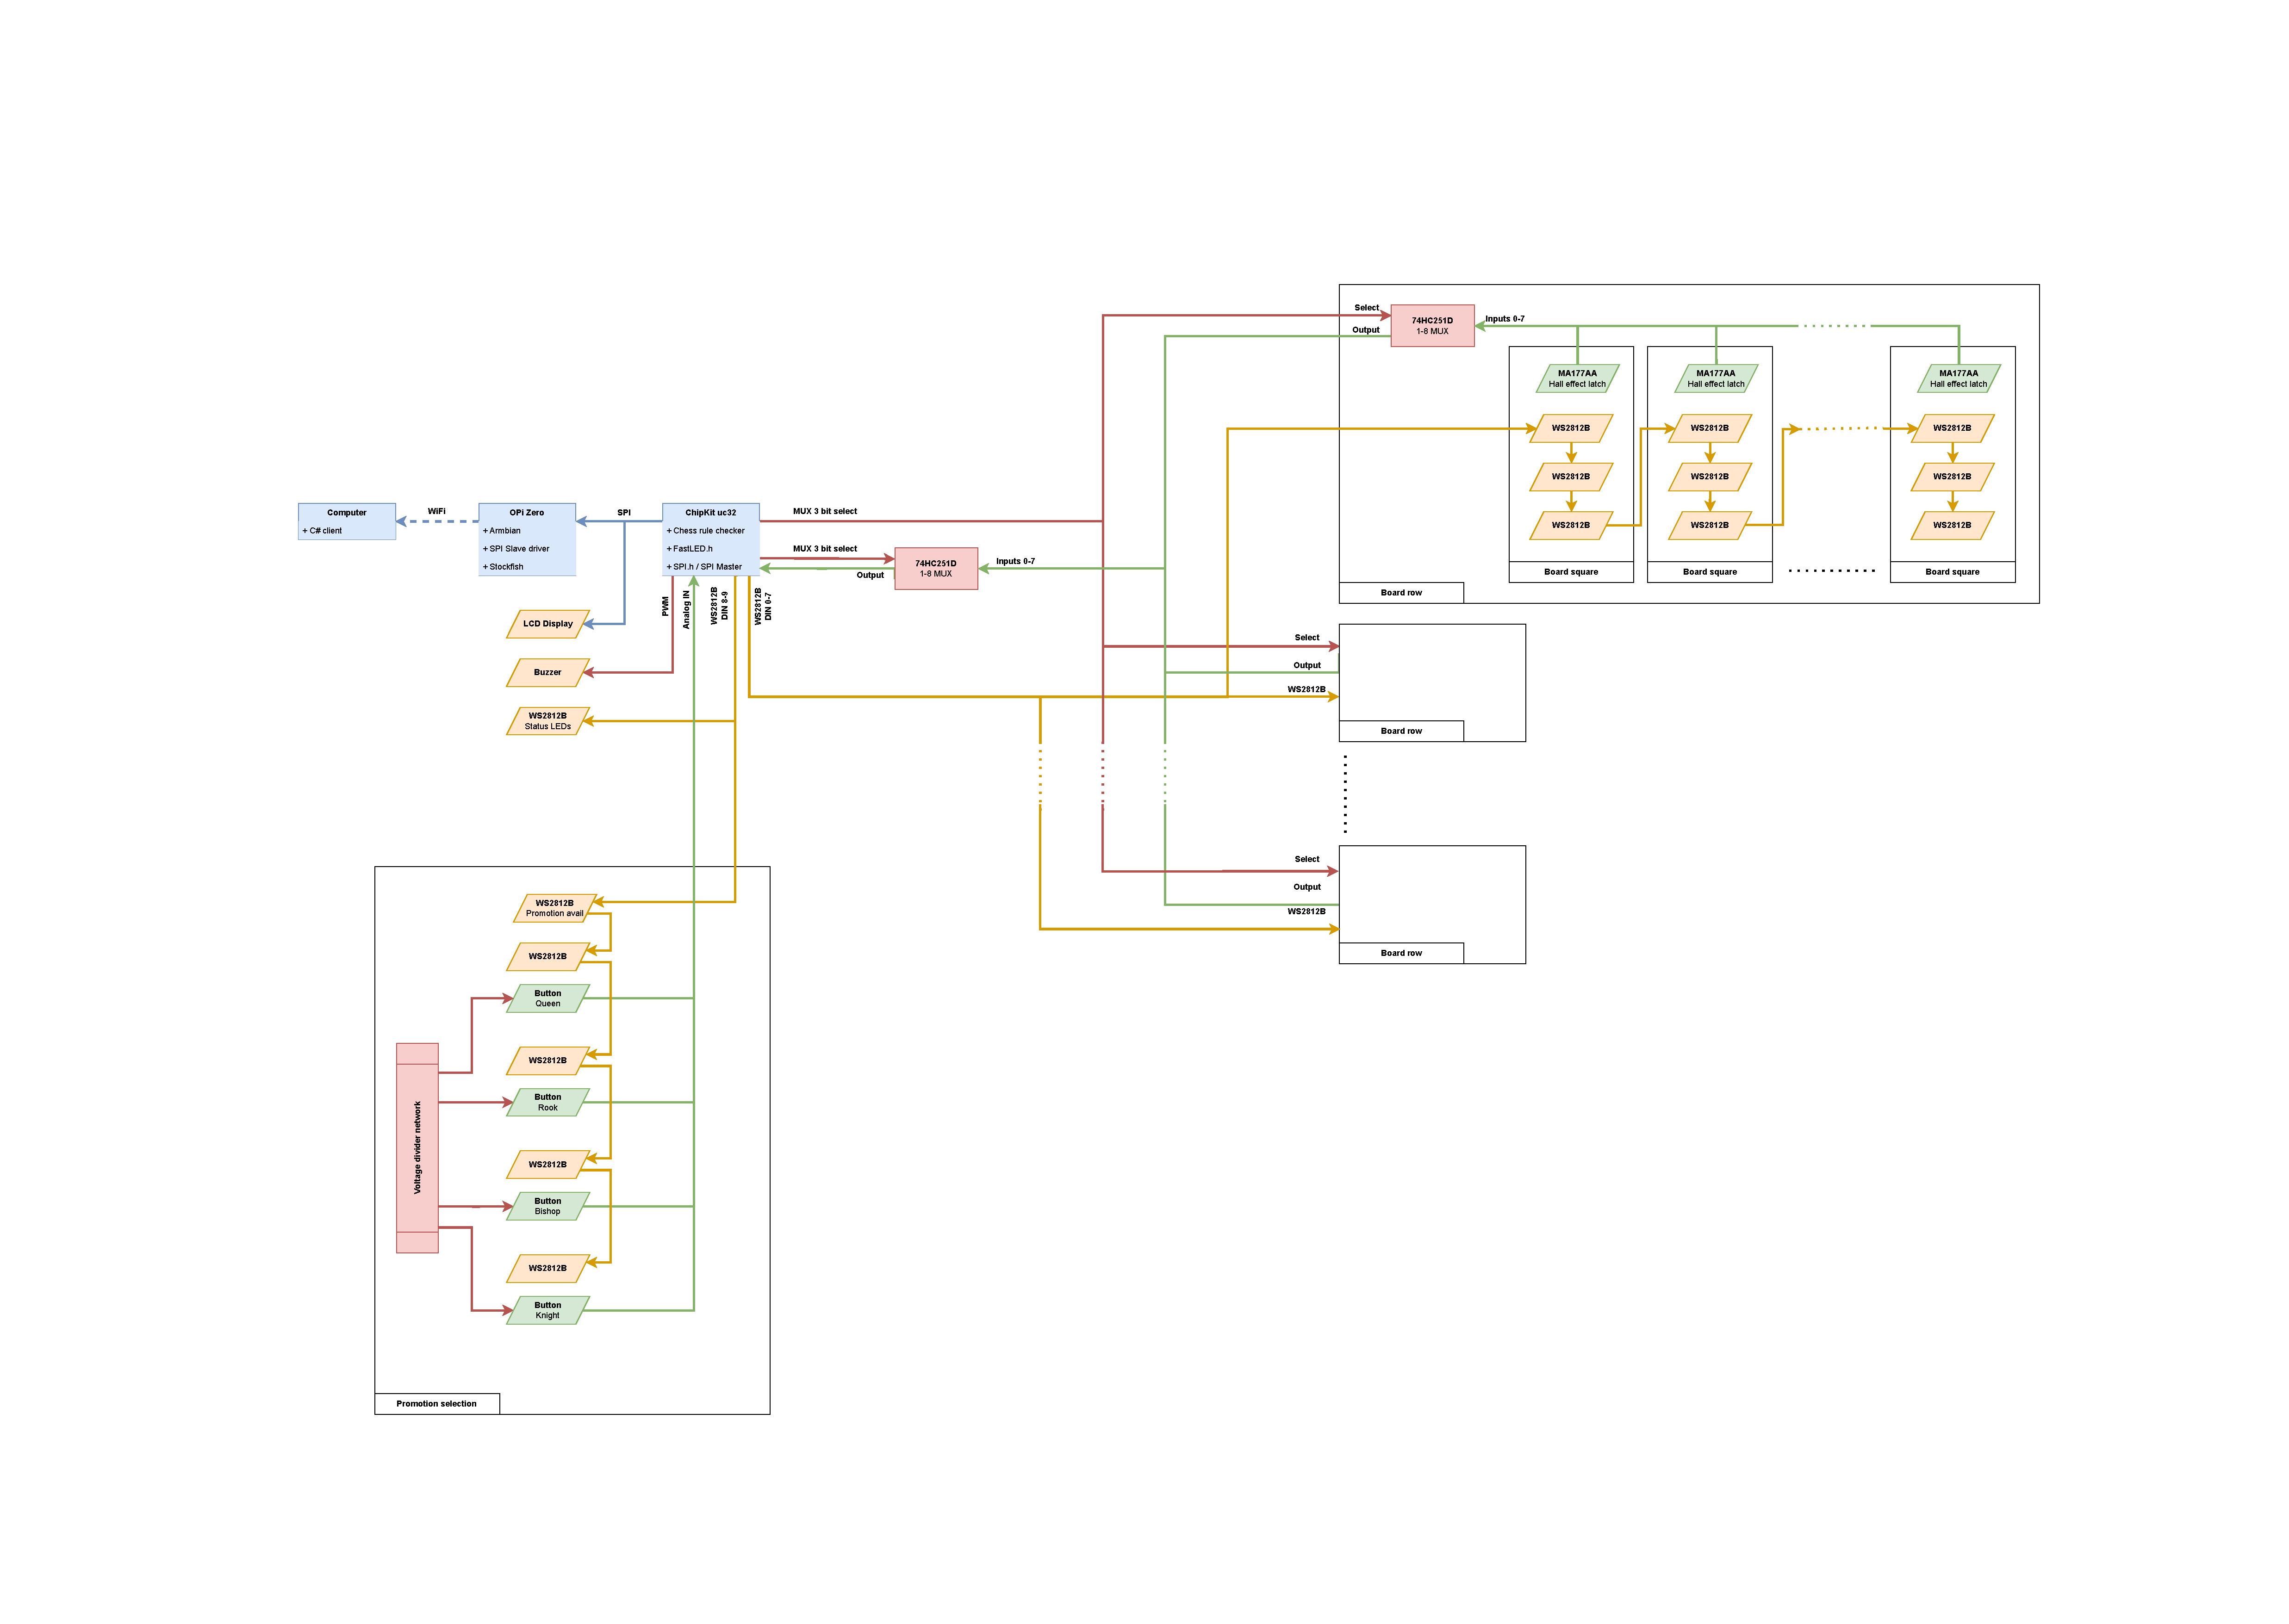
\includepdf[pages=-,angle=90]{appendix/digichess_architecture.pdf}
		\end{figure}
	\end{landscape}

	\section{Draft model of the chessboard face}
	\section{Cross-section view of a square's piece slot}
	\section{Board module PCB}
\end{appendices}

\end{document}